\section{Contexte historique}
    \subsection{La Chine impériale sous la dynastie Qing}

Le projet \COREL vise à étudier l'évolution du droit lors de la période de la Chine impériale tardive, de 1644 à 1911. Ces bornes chronologiques correspondent au règne de la dynastie Qing. En effet, les Qing, venant de Mandchourie, renversent la dynastie Ming (1368-1644) en prenant la capitale, Pékin. La dynastie Qing règne alors avec l'empereur Shunzhi (1644 - 1661) au pouvoir, lequel opère la transition entre les deux dynasties. Il fait éditer le premier code légal des Qing, le \dqlj, qui hérite directement du code des Ming, révisé pour la nouvelle dynastie. La modification du code légal de la dynastie précédente, selon Zheng Qin et Guangyuan Zhou, s'explique ainsi : 

\begin{quote}
    Indeed, the relatively smooth transition
 from the Ming code to the Qing code needs some explanation. The
 Ming code represented the highest legislative achievement in tradi-
 tional China, making the new rulers reluctant to abandon it. Further-
 more, the Manchu rulers had already familiarized themselves with the
 Ming law and political system before they conquered China. \footnote{\cite{qin_pursuing_1995}}
\end{quote}
C'est donc dans la continuité directe du code des Ming que va s'écrire le code légal des Qing.

Après Shunzhi, c'est l'empereur Kangxi (1662-1722) qui est à la tête du pays. Son règne se caractérise par une certaine ouverture aux sciences occidentales via des jésuites, venus en Chine pour transmettre leurs savoirs et tenter d'évangéliser la Chine. L'empire Mandchou s'étend progressivement jusqu'au milieu du XVIII\ieme siècle. Deux autres grands empereurs succèdent à Kangxi : Yongzheng (1723 - 1735) et Qianlong (1736 - 1795). En 1911, la dynastie Qing est remplacée par un gouvernement républicain.

\subsection{La législation chinoise et l’édition des codes légaux}

Les textes de lois chinois relèvent majoritairement du droit pénal et observent une structure définie et rigoureuse. Sous la dynastie des Qing, les codes légaux se divisent en sept chapitres majeurs (appelés \textit{bu}), structure déjà employée pour les textes de lois de la dynastie précédente. En effet, le code des Ming de 1397 utilise cette division en sept chapitres, dont les codes des Qing héritent. Le premier chapitre contient des propos généraux (\og Dénominations et règles \fg \footnote{Les titres de chapitres, entre guillemets, sont empruntés à la traduction proposée par le projet \LSC.}) et les six chapitres suivants sont organisés selon les six ministères (la division du gouvernement en ces six ministères étant observée depuis la dynastie Tang \footnote{Dynastie régnante en Chine de 618 à 907}) : \og Lois administratives \fg, \og Lois domestiques \fg, \og Lois rituelles \fg, etc. À l'instar du code des Ming, ces chapitres sont ensuite divisés en trente sections (en chinois \textit{men}), par exemple \og Institutions administratives \fg, \og Documents officiels \fg, etc. 

Ces chapitres et sections contiennent deux types de lois. Les lois dites principales, les \lu, sont des lois fixes qui constituent la colonne vertébrale du code des Qing (en anglais \textit{statutes}). Certaines lois principales sont directement héritées de la législation de la dynastie Tang, ou ont subi des changements mineurs de vocabulaire. Selon Derk Bodde et Clarence Morris, fixer des lois immuables d'une dynastie à l'autre relèverait d'une vision morale de la loi en Chine : 
\begin{quote}
    No doubt this continuity reflects the Chinese view of law as the codification of moral truths retaining eternal validity irrespective of time or place. \footnote{\cite{law_in_imperial_china}}
\end{quote}

Toutefois, ce propos est nuancé dans leur ouvrage puisque, de fait, moins de la moitié des lois principales demeurent véritablement immuables. Les autres \lu sont modifiées, parfois supprimées ou même créées sous la dynastie Qing, jusqu'en 1740, année de leur dernière version. De plus, les \lu sont accompagnées d'articles additionnels (ou lois secondaires), les \li (aussi appelées \textit{li}, ou en anglais \textit{substatutes}). Les lois secondaires sont des ajouts aux lois principales. Loin d'être figées, elles traitent du droit vivant et viennent préciser la loi principale à laquelle elles sont rattachées. Elles apparaissent souvent à la suite de jugements ou de cas particuliers. Les lois principales ont tendance à se réduire avec le temps. Elles sont au nombre de 436 en 1740. En revanche, les \li augmentent au fur et à mesure. Il en existe une centaine en 1740. À la fin du XIX\ieme siècle, on compte plus de 1 000 lois secondaires. 

 \section{Des sources juridiques}
    \subsection{Les éditions du code légal (1646, 1740)}

Les codes légaux des Qing sont révisés et publiés de manière plus ou moins régulière, tous les dix ans environ. Entre 1740 et 1871, date de la dernière édition du code, on compte 23 rééditions. Toutefois, toutes ces rééditions n'ont pas été conservées, ce qui laisse le corpus incomplet. Dans le cadre du projet \COREL, deux éditions du code légal sont utilisées. 

En 1646, la première édition du code légal des Qing, \dqlj, compte une centaine d'articles. Cette première édition du code s'inscrit dans la continuité du code de la dynastie Ming. Les historiens, notamment Tan Qian  qui a connu les deux dynasties, critiquent cette première édition du code qui n'a pratiquement rien de nouveau et ressemble très fortement au code des Ming. 

La seconde édition du code des Qing intégrée au corpus du projet est le code de 1740, \dq. Dans cette version du code, les \lu sont définitivement établies et ne sont plus modifiées. Comme son nom l'indique, ce texte met sur le même plan les lois principales, \lu et les lois secondaires, \li. En effet, sous la dynastie Ming, les \li n'étaient que des exemples aux lois principales. Elles prennent de plus en plus d'ampleur dans le droit chinois, jusqu'à avoir véritablement la même importance que les lois principales en 1740.

Néanmoins, ces éditions du codes, largement espacées, ne reflètent la loi qu'au moment où elles sont produites et ne prennent pas en compte les modifications qu'il y a pu y avoir entre deux éditions. C'est pourquoi, en plus des éditions des codes légaux, d'autres sources viennent nourrir le projet \COREL : des compilations des textes de lois, qui viennent compléter les zones d'ombres que laissent les codes légaux.

\subsection{Les compilations des textes de loi}

Les compilations des textes de lois sous la dynastie Qing ont une structure similaire à celle des codes légaux et suivent la structure rigoureuse en sept chapitres. Toutefois, ces documents présentent également des caractéristiques qui leur sont propres et viennent compléter les codes légaux. 

En 1871, le \genyuan est publié. Il présente les articles additionnels dans l'ordre chronologique, c'est-à-dire dans l'ordre de modification du code légal. Le \huidian paraît en 1899 et compile l'ensemble des lois en vigueur mais aussi les lois abrogées. Enfin, le \dc est un texte de 1905 qui compile toutes les lois en vigueur sous la dynastie des Qing, avec des explications historiques. Cette compilation a été établie par Xue Yuncheng pour aider à la révision du code légal. Ces trois textes sont des sources qui viennent compléter les textes légaux grâce à leur exhaustivité en présentant toutes les modifications et abrogations des lois et permettent d'en retracer la généalogie.

En plus de ces textes, il existe des recueils de cas qui expliquent l'origine des lois. En effet, les articles additionnels résultent de jugements ou de cas particuliers, il est donc possible de retracer l'origine d'une loi à une affaire, un décret ou un fonctionnaire. Toutefois, ces documents ne font pas partie du projet \COREL. Actuellement en cours de numérisation par la bibliothèque d'études chinoises, les informations supplémentaires que peuvent apporter ces sources constituent une perspective d'enrichissement des données du projet qui sera envisagée à termes. 


\section{Les sources numériques}
    \subsection{Les documents \XML}
Le projet \COREL dispose de sources numériques issues des projets précédents. Ces sources ont été pensées et produites pour deux projets différents et ne sont pas liées entre elles. La source de données principale du projet provient du projet \LSC, qui offre une édition en ligne des sources balisées en \XML. 

\subsubsection{Encodage et validation des données}
Ce balisage \XML relève d'un schéma personnalisé, créé spécifiquement pour le projet \LSC. Pour comprendre ce balisage, il est indispensable de consulter en regard l'édition \XML et le site web du projet, qui sont étroitement liés. En effet, le balisage reprend la structure des codes légaux, familière aux chercheurs, mais lie ce balisage à l'affichage \HTML. Ainsi, certaines portions des textes sont balisées ainsi : 
\begin{minted}{xml}
<p>笞刑五:
    <inf>笞者,擊也,又訓為恥。用小竹板。</inf>一十;
    <inf>折四板。</inf>二十;<inf>除零,折五板。</inf>三十;
    <inf>除零,折一十板。</inf>四十;
    <inf>除零,折一十五板。</inf>五十;
    <inf>折二十板。</inf>
</p>
\end{minted}

En comparant ce code \XML à l'affichage du site, il est possible d'établir clairement le lien entre l'encodage et l'affichage : la balise \texttt{<inf/>} permet d'afficher une partie des paragraphes en caractères bleus, dans une police légèrement inférieure. 
\begin{figure}[h]
    \centering
    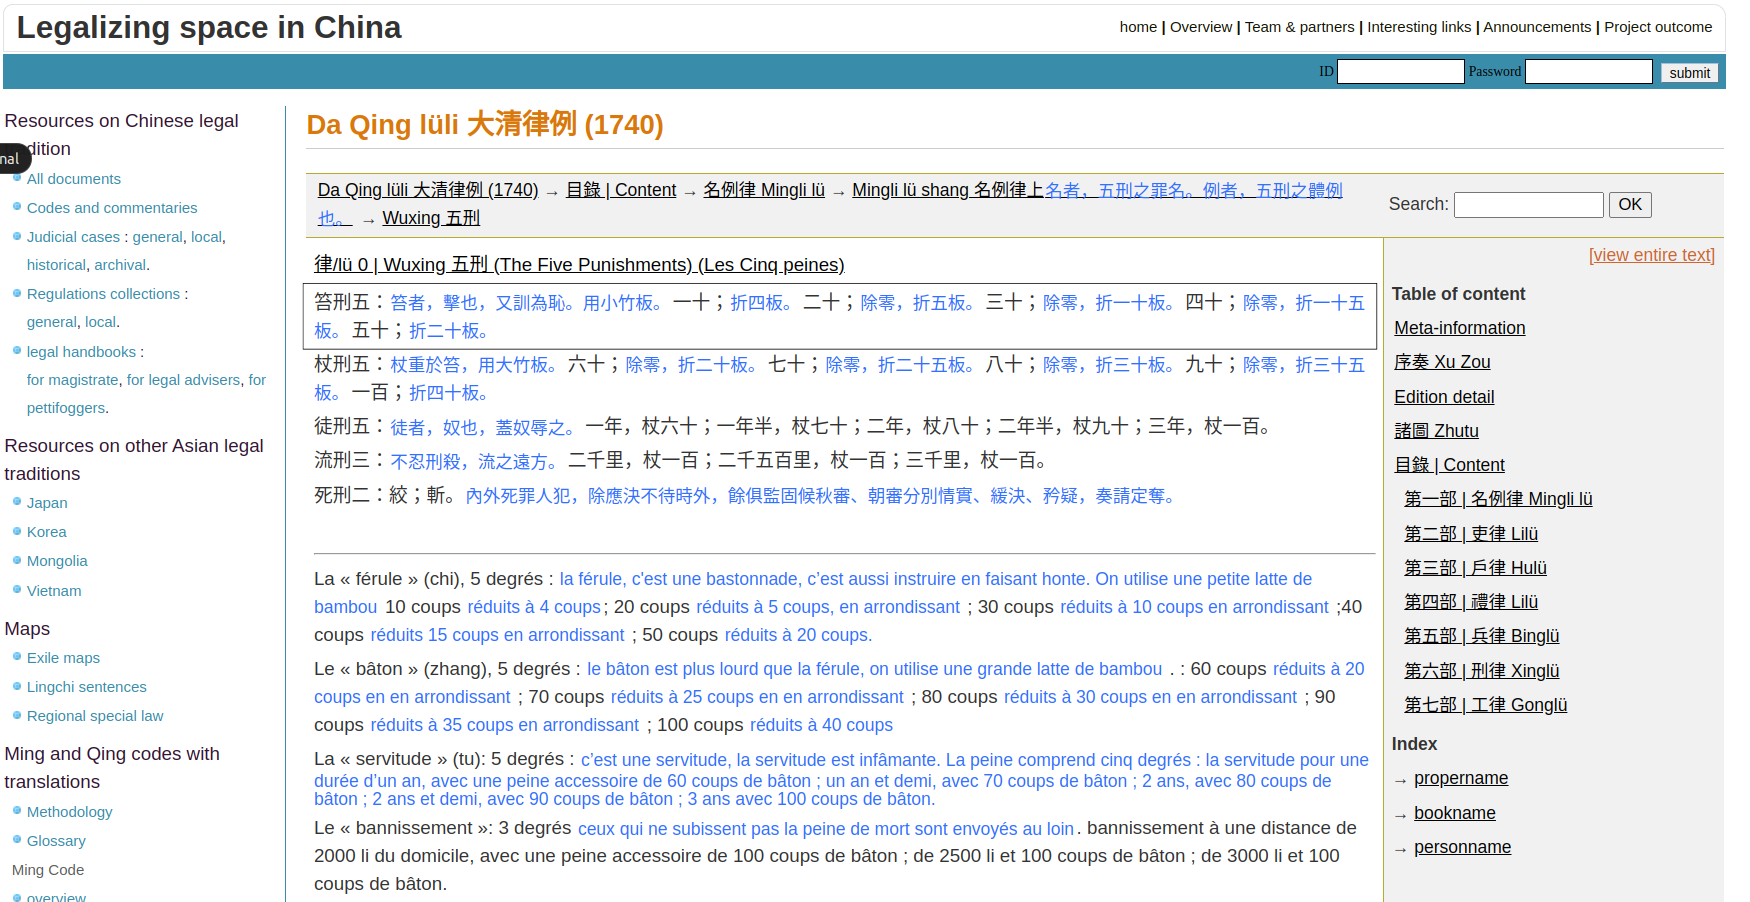
\includegraphics[width=\textwidth]{images/image1.png}
    \caption{Capture d'écran du site web \LSC - affichage du code \XML dans l'encadré.}
\end{figure}

Cette utilisation de l'encodage relève du mode de travail des chercheurs sur le projet. En effet, à partir de textes issus de l'\OCR, le texte est saisi et balisé dans le logiciel Oxygen au fur et à mesure du projet, c'est-à-dire que l'encodage des données et le développement du site s'effectuent en parallèle. Dès lors, le site web devient un outil de validation de la saisie des données : ce lien entre l'encodage et l'affichage permet aux chercheurs débutants en humanités numériques de vérifier leur code en mettant le site à jour, les erreurs d'affichages se repérant plus facilement qu'un oubli dans le code \XML. 

Mettre en parallèle les étapes d'encodage et de création du site internet relève du choix des chercheurs du projet d'utiliser un schéma \XML entièrement customisé. En effet, ce schéma n'est pas documenté et aucune \DTD n'a été produite pour valider l'encodage et contraindre ce schéma. Le projet \LSC continue aujourd'hui d'être alimenté par les chercheurs du projet \COREL. Dès lors, le seul moyen de se repérer dans un schéma sans documentation ni règles de validation devient l'affichage du site internet.

\subsubsection{Structure des sources numériques}
Sans documentation claire ni schéma de validation, comprendre la structure des sources numériques et les choix d'encodage est une étape essentielle du projet. En effet, il est difficile de comprendre au premier coup d'oeil le schéma utilisé pour encoder les sources sans avoir travaillé pour le projet \LSC et sans connaissances solides des textes de lois chinois. De plus, au fil du temps, les sources numériques ont été encodées par de nombreuses personnes, contribuant au projet \LSC ou bien au projet \COREL. L'encodage n'étant pas contraint et les objectifs des deux projets étant différents, les sources numériques ont parfois évolué et l'encodage des texte peut présenter des variantes d'encodage d'un texte à l'autre, voire au sein d'un même document. 

L'encodage \LSC prend comme point de départ la structure des sources originales en chapitres, sections, lois principales et secondaires, mais vient ajouter des éléments supplémentaires selon les spécificités de chaque document. Par exemple, le \huidian propose des listes de lois classées par année. Cet élément est propre à ce texte de lois et a nécessité un encodage différent, traduit par un élément \texttt{<enum>} contenant un ou plusieurs \texttt{<item>} et une balise \texttt{<date>}.

De plus, le projet \LSC est un projet d'édition scientifique numérique trilingue. Tous les documents ont donc été encodés en chinois, français et anglais. Chaque balise apparaît donc trois fois, avec un attribut de langue différent. 
\begin{minted}{xml}
    <title lang="ch">Wuxing 五刑</title>
    <title lang="en">The Five Punishments</title>
    <title lang="fr">Les Cinq peines</title>
\end{minted}
Toutefois, ces choix manquent d'uniformité dans l'encodage, car certaines balises ne sont pas triples et contiennent des informations hybrides entre plusieurs langues :
\begin{minted}{xml}
    <title lang="ch">目錄 | Content</title>
\end{minted}
D'autre part, la traduction des textes n'a jamais été achevée pendant le financement du projet \LSC. Il existe ainsi de nombreuses balises auto-fermantes dans l'encodage \XML, qui laissent la place à une traduction qui n'a pas de garantie de voir le jour, d'autant plus que le projet \COREL n'inclut pas les traductions dans son périmètre. 

Le trinlinguisme initial du projet \LSC semble à première vue être un élément que l'on peut aisément écarter du projet \COREL. Toutefois, il a des conséquences directes dans l'encodage. En effet, outre les nombreuses balises auto-fermantes qui rendent le code dense, il est possible d'observer une substitution progressive entre la balise \texttt{<content>} censée séparer les différentes traductions et la balise \texttt{<p>} qui permet de séparer les différents paragraphes. Puisque la balise \texttt{<content>} n'est pas effective dans le cadre du projet \COREL et systématiquement laissée vide pour le français et l'anglais, son utilisation première s'est parfois perdue et s'est substituée à la balise \texttt{<p>} lorsque le texte chinois ne contenait qu'un seul et unique paragraphe. 

Par ailleurs, le choix d'éditer des documents trilingues s'est aussi reflété dans la création du schéma d'encodage. Si les éléments les plus courants, comme les titres, possèdent des noms de balises en anglais, ce n'est pas le cas de la plupart des éléments structurants des sources. Ainsi, les chapitres sont balisés grâce à l'élément \texttt{<bu>}, les sections \texttt{<men>}, etc. Certaines balises viennent également rappeler le français, comme la balise \texttt{<inf>} qui vient signaler des caractères de police \textit{inférieure}. 

Tous ces éléments aboutissent à la création de sources numériques extrêmement spécifiques et viennent restreindre la communauté qui peut contribuer au projet ou en bénéficier, car seules quelques personnes possèdent toutes les clefs de compréhension pour déchiffrer ce support de travail. 

\subsection{La numérisation des codes légaux}
\subsubsection{\IIIF et annotations}
En plus des données produites par le projet \LSC, le projet \COREL hérite aussi des sources produites par le projet \EPJ. Les numérisations des textes de lois ont été déposées sur un serveur \IIIF géré par Data Futures. Les chercheurs ont ensuite accès à un visualiseur Mirador qui leur permet de segmenter les images pour expliciter la structure des codes légaux en chapitres, sections, \lu et \li. Cette segmentation permet de mettre en valeur un caractère annonçant le début d'une nouvelle partie. 

\newpage
\begin{figure}[h]
    \centering
    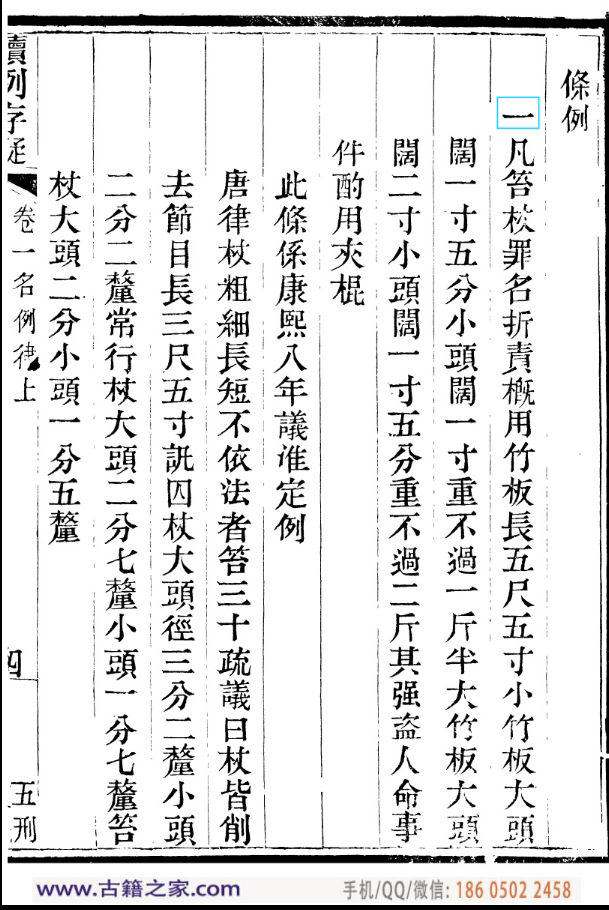
\includegraphics[width=100mm]{images/image2.png}
    \caption{Numérisation du \dc, segmentation du début du \li 1-1}
\end{figure}

Ces caractères qui marquent le début d'un élément structurant du document ont ensuite été annotés par les chercheurs. Le prestataire a mis en place un tableau à remplir pour annoter les passages segmentés. 

\begin{figure}[h]
    \centering
    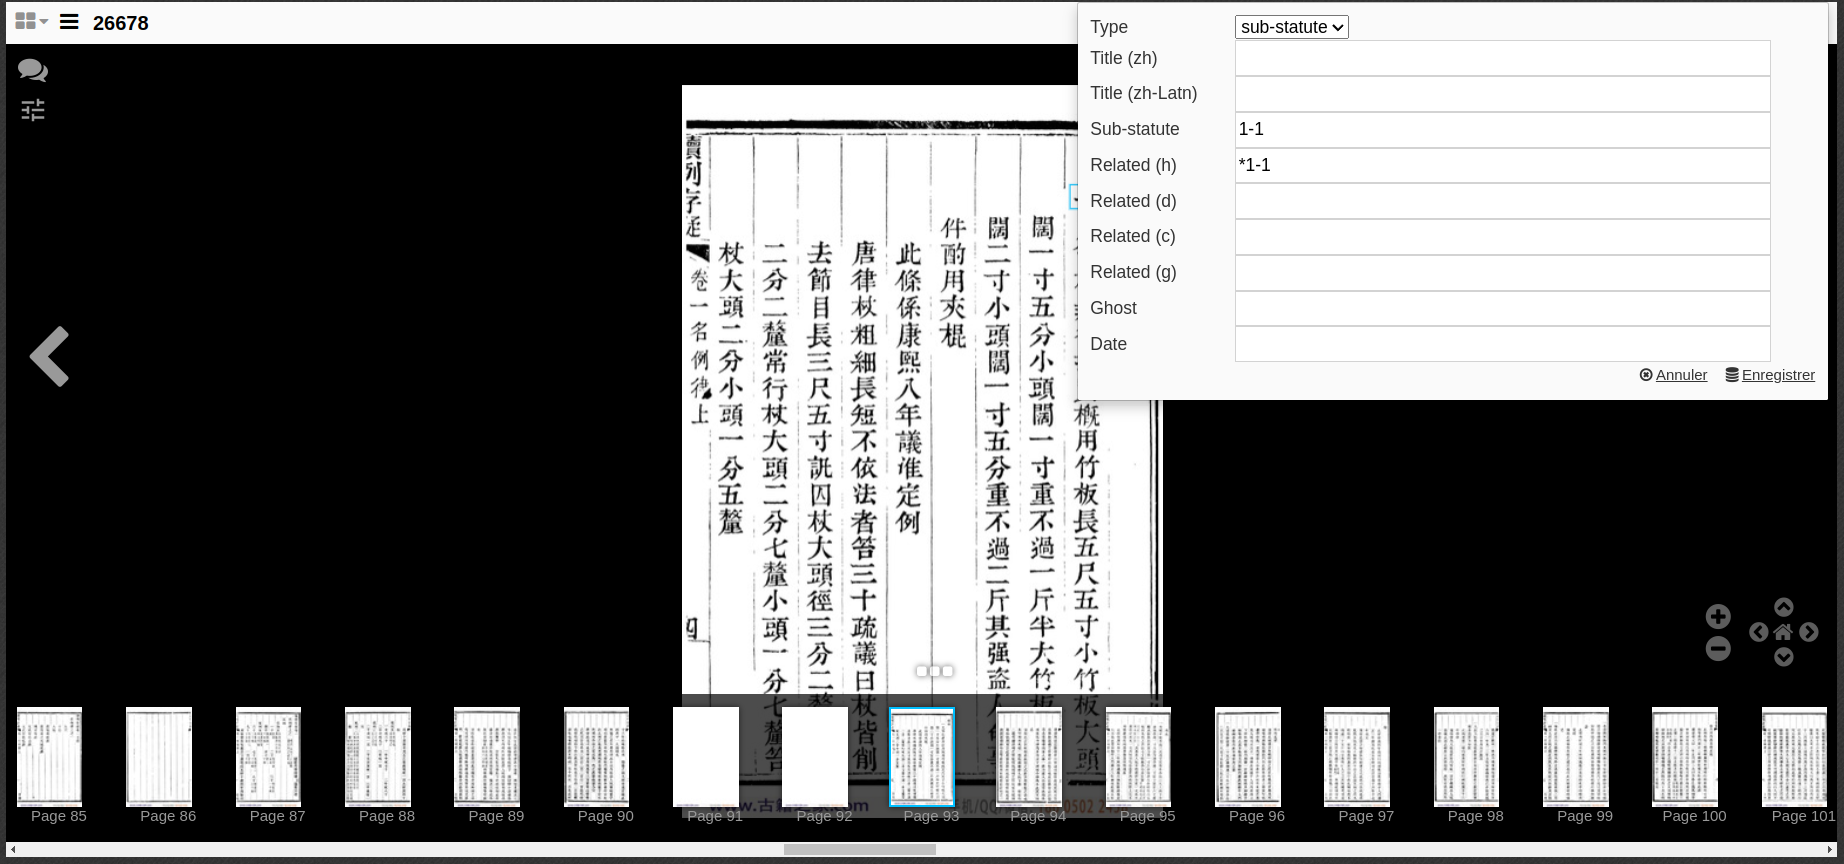
\includegraphics[width=\textwidth]{images/image3.png}
    \caption{Interface d'annotation du visualiseur Mirador}
\end{figure}
Cette pratique a permis aux chercheurs de produire des annotations structurées et uniformes d'un texte à l'autre. Dans ce cadre figurent notamment des informations sur la date de début de validité des lois et des liens de généalogie. 

\newpage
\subsubsection{Généalogie des lois}
Ce travail d'annotation et de segmentation des textes, toujours en cours en parallèle du projet \COREL, a pour objectif de retracer la généalogie des lois. Les annotations sont remplies à partir d'un référentiel. Ce référentiel prend comme source de départ le \genyuan. C'est un fichier texte disponible en ligne, hébergé par Data Futures. Il recense chaque loi une à une, généralement avec le lien vers la numérisation correspondante, et indique deux types de liens. Le premier est un lien d'association simple. Il indique les correspondances entre la loi du \genyuan à une loi d'un autre document. 
\begin{figure}[h]
    \centering
    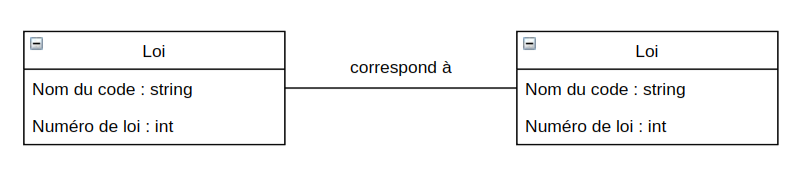
\includegraphics[width=\textwidth]{images/image4.png}
    \caption{Modélisation d'un lien d'association entre deux lois}
    \label{Modélisation d'un lien d'association entre les lois}
\end{figure}

Ce lien d'association simple est à indiquer dans les rangs \textit{related} des annotations. Elles indiquent les lois associées à celle de l'image dans les autres textes de lois, chaque lettre correspondant à une source textuelle différente : h pour \huidian, g pour \genyuan, d pour \dc et c pour \dq. 

Le référentiel indique également un deuxième type de lien, qui n'est pas présent dans les annotations des images. C'est un lien d'association dirigée, qui indique des liens de généalogie entre les lois. Pour distinguer ces liens de généalogie des liens d'association simple, les chercheurs ont mis en place dans le référentiel un vocabulaire spécifique à ces liens. Les liens \og \textit{in} \fg indiquent qu'une loi est issue d'une autre, et les liens \og \textit{out} \fg indiquent qu'une loi donne naissance à une autre.

\begin{figure}[h]
    \centering
    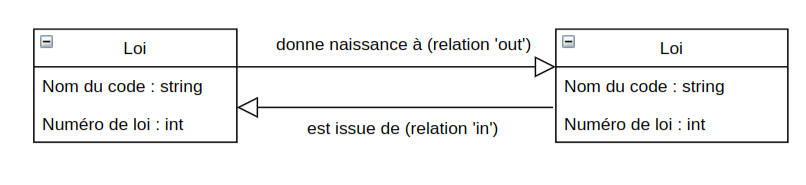
\includegraphics[width=\textwidth]{images/image5.png}
    \caption{Modélisation des liens d'association dirigée entre deux lois}
\end{figure}

Lorsque les informations du référentiel sont retranscrites dans les annotations, elles sont stockées dans des fichiers \JSON que le prestataire fournit à l'équipe du projet. Toutefois, ces données ne sont que partiellement accessible car le projet dispose uniquement des fichiers correspondant aux annotations, sans le manifeste \IIIF, ne donnant pas accès aux métadonnées, lesquelles sont accessibles uniquement via une plateforme gérée par Data Futures aux utilisateurs connectés. Cet accès se fait uniquement en interface graphique, ces données ne sont donc pas exploitables. De plus, l'annotation des images étant toujours en cours de saisie, les fichiers \JSON sont encore incomplets, puisque les valeurs ne sont pas encore entièrement saisies. Dans cet exemple, la date de début de validité de la loi n'a pas encore été saisie. 

\begin{minted}{json}
    {
            "chars" : "",
            "format" : "text/plain",
            "@type" : "freizo:date"
         },
         {
            "chars" : "254",
            "@type" : "freizo:number"
         },
\end{minted}

Ces données, en plus d'être partielles et toujours en cours de saisie, contiennent parfois des informations qui sont encore à expliciter. C'est notamment le cas du champ de date des annotations. À l'intérieur de celui-ci, les chercheurs entrent la date de début de validité d'une loi. Pour retrouver la date de fin, il est nécessaire de passer par les liens de généalogie. À partir d'un lien \textit{in}, il faut alors déduire que la date de début d'une loi B met fin à la période de validité d'une loi A. 

Les données à disposition du projet \COREL sont donc entièrement issues des deux projets précédents. Pensées et produites à des fins différentes, ces sources numériques ne sont pas liées entre elles, en plus d'être produites dans des formats différents. 
